\chapter{Revisão Bibliográfica}

\resumodocapitulo{Neste capítulo, apresentamos uma revisão bibliográfica de \acrshort{codec}'s de imagem desenvolvidos com técnicas de redes neurais artificiais. O autocodificador é uma \acrshort{rna} presente na maioria dos trabalhos. As diferenças estão na arquitetura dos autocodificadores, na modelagem do problema, emprego de análises probabilísticas, generativas, de segmentação semântica, etc.}  
%Otimização conjunta de taxa e distorção é difícil. Sem maiores restrições, o problema geral da quantização ótima em espaços de alta dimensão é intratável (
%Os \acrshort{codec}'s artesanais tradicionais carecem de adaptabilidade e são incapazes de aproveite a redundância semântica em imagens naturais. 
\section{Introdução}

%Por exemplo, o \acrshort{jpeg} realiza a \acrshort{dct} e a decomposição ortogonal em várias escalas de \acrshort{wavelet} é usada pelo JPEG2000.
As técnicas de redes neurais para compressão de imagens é um tema que vem despertando o interesse de muitos pesquisadores e já apresenta resultados competitivos com o \acrshort{bpg} (considerado o estado da arte de compressão de imagens) em alguns trabalhos \cite{Priming2017Johnston,Autoregressive2018Minnen,akbari2019dsslic}. 

Há 3 principais abordagens para incluir \acrshort{rna}'s na tarefa de compressão de imagens \cite{Jiang1999}. A primeira é o desenvolvimento completo do par codificador-decodificador. A segunda consiste na implementação de redes neurais dos algoritmos tradicionais de compactação de imagem. A terceira abordagem é usar uma \acrshort{rna} para substituir, aperfeiçoar ou adicionar alguma etapa na compressão de imagens realizadas por \acrshort{codec}' conhecidos. Aqui, o objetivo é fornecer melhorias adicionais a esses algoritmos \cite{Jiang1999}. Hoje, a primeira abordagem é a predominantes e vem obtendo os melhores resultados.

O problema central na compressão de imagens com perdas é a otimização conjunta da taxa e distorção. Esse objetivo se torna intratável para imagens ou espaços de alta dimensão sem a imposição de alguma restrição \cite{gersho2012vector}. Devido a isso, os \acrshort{codec}'s tradicionais aplicam transformações lineares para gerar uma representação adequada sobre a qual podemos considerar a otimização conjunta de distorção e taxa \cite{End2016Balle}. Entretanto, não há razão para esperar que uma função linear seja ideal para comprimir todo o espectro de imagens naturais e ainda considerando os formatos de mídia emergentes \cite{santurkar2018generative}.  

As abordagens baseadas em \acrshort{rna} \cite{Variable2016Toderici,Priming2017Johnston,target,Priming2017Johnston,FullResolution2017Toderici,End2016Balle,Autoregressive2018Minnen,Lossy2017Theis,Variational2018Balle,zhao1901cae} substituem as transformações lineares por funções básicas aprendidas capazes de aprender recursos das imagens. Nesses trabalhos, a arquitetura do autocodificador contém ao menos uma  camada não-linear, e o modelo como um todo é não-linear.   


%Todas essas abordagens baseadas em ML seguem uma estrutura semelhante de autoencoder, em que um codificador é usado para extrair representação de recursos de imagens e um decodificador é responsável por reconstruir imagens das representações quantizadas. As principais diferenças entre essas abordagens baseadas em ML são as arquiteturas de codificador e decodificador. Enquanto a maioria desses algoritmos [33, 36, 17, 19, 37, 20] emprega CNNs como codificador e decodificador, outros exploram redes recorrentes, como LSTM e GRU [34, 35].










%Uma das vantagens do uso de \acrshort{rna}'s para a compressão de imagens é a facilidade de adaptação da rede para que possa comprimir eficientemente novas mídias (imagens não-naturais).  %É razoável pensar no uso de IA para tarefa de compressão de imagens.

%A natureza da compressão com perdas pressupõe a utilização de quantização dos dados. Tal operação não é diferenciável e impõe uma restrição ao uso de \acrshort{rna} para a compressão.

%Outra preocupação é fornecer ao \acrshort{codec} flexibilidade similar aos  tradicionais de imagens. Em geral, deseja-se que a rede seja capaz de fornecer reconstruções progressivas, controlar a qualidade e a taxa, codificar e decodificar  em tempo similar os \acrshort{codec}'s convencionais, etc.

%Na literatura, os autocodificadores se popularizaram como uma rede neural capaz de realizar compressão de dados.  Como já apresentado é uma abordagem fim-a-fim que pode ser adaptada para as tarefas de compressão de imagens.


\section{Autocodifcadores em cadeia}
Nessa seção, apresentamos trabalhos que usam arquiteturas baseadas em cascateamento de autocodificadores para compressão de imagens. Várias camadas de \acrshort{rna} são testadas na tentativa de aprimorar a peromance do modelo.   


Em \cite{Variable2016Toderici}, Toderici et. al propuseram arquiteturas de redes neurais voltados para compressão de imagens em miniaturas. As arquiteturas são baseadas no uso de autocodificadores encadeados e treinadas pelas imagens e suas informações residuais obtidas progressivamente. 
Esse encadeamento pode ser explícito, isto é, todos os autocodificadores foram explicitamente definidos, portando, cada um possui seus próprios pesos e camadas. 
No encadeamento implícito apenas um autocodificador é projetado, porém, durante a execução do modelo, conexões de retroalimentação são realizadas nesse autocodificador. Assim temos um cascateamento devido ao \textit{loop}, onde os pesos do autocodificador são compartilhados nas iterações. O número escolhido de autocodificadores (implícitos ou explícitos)  definem a quantidade de iterações do modelo. 

Durante a execução (treinamento ou teste) de qualquer uma das arquiteturas apresentadas em \cite{Variable2016Toderici} a primeira iteração segue o seguinte procedimento: toma uma imagem $x = r_0$ passa pela função $E_1$ (codificador 1), o resultado é transformado em códigos binários por uma função $B$ (função de binarização), em seguida a rede do decodificador $D_1$ (decodificador 1) cria uma estimativa da imagem de entrada original com base no código binário recebido. Então, calcula-se o resíduo da primeira iteração, dado por $r_1 = r_0 - D_1(B(E_1(r_0)))$. 
Na próxima iteração, o $E_2$ recebe a informação residual e uma  saída é gerada por $D_2$.   Entretanto,  a nova saída nessa iteração e das próximas, podem ser a informação residual reconstruída ou uma nova versão da imagem original (reconstrução única), como veremos.  Após o modelo realizar o número defnido de etapas, passamos a processar a próxima imagem e o ciclo se repete. 

Podemos resumir a ideia do encadeamento de autocodificadores com a próxima Equação: 

\begin{equation}
\begin{aligned}
F_t(r_{t-1}) &= D_t(B(E_t(r_{t-1}))) \\
\end{aligned}
\end{equation}

onde $E_t$ e $D_t$ são o codificador e decodificador da iteração $t$-ésima para a qual $ r_{t-1}$ é a entrada. A função de binarização $B$ é o mesmo em todas as iterações. A equação para obter o resíduo $r_t$ depende da informação de saída do autocodificador $F_t$.  Os pares codificador-decodificador são treinados de ponta a ponta, mas durante a implantação, eles são normalmente usados independentemente.

Antes de apresentar os modelos com mais detalhes, discutiremos o processo de binarização adotado.


\subsection{Binarização}
\label{subsec:bin}

%A binarização consiste em um mapeamento de valores em ponto flutuante para o intervalo $[- 1, 1]$. Ela é equivalente a função de ativação limiar descrita na Tabela \ref{table:func_ativacoes}. Logo, tal operação possui derivada nula ou indefinida.  Por isso, é necessário uma manipulação para que possam treinar uma rede neural com uma camada de binarização.
%A primeira parte é a geração de valores no intervalo contínuo $[- 1, 1]$. A segunda parte envolve a conversão desses valores para o conjunto discreto $\{- 1, 1\}$.


O trabalho \cite{Variable2016Toderici} propõe uma operação de binarização e um método para transpor a limitação que esse processo impõe ao treinamento de uma \acrshort{rna}. 
Nessa proposta, uma camada totalmente conectada com ativação de $\tanh$ é usada para produzir as saídas no intervalo contínuo $[1,-1]$. Em seguida, uma abordagem estocástica usada durante o treinamento da rede é aplicada para converter desses valores para o conjunto discreto $\{- 1, 1\}$. Sendo $x$ um valor a ser quantizado e $\epsilon$ o erro de quantização devemos ter.

\begin{equation}
\begin{aligned}
b(x) &= x + \epsilon  \\
b(x) & \in \{-1, 1\}
\end{aligned}
\end{equation}

O valor $\epsilon$ é obtido dentre dois valores possíveis e obedece a seguinte regra estocástica:

\begin{equation}
\label{eq:quant2}
\begin{aligned}
\epsilon \sim \left\{
\begin{array}{ll}
1 - x, \text{com probabilidade } \frac{1 + x}{2} \\
-x - 1, \text{com probabilidade} \frac{1 - x}{2}
\end{array}
\right. \\
\end{aligned}
\end{equation}

Na prática, definimos um valor $u$ entre 0 e 1 obtido de uma distribuição uniforme, isto é,  $u \in \mathcal{U}[0,1]$ e podemos reescrever \ref{eq:quant2} como:

\begin{equation}
\label{eq:quant}
\begin{aligned}
\epsilon \ = \left\{
\begin{array}{ll}
1 - x, \text{ se $u$}  \leq \frac{1 + x}{2} \\
-x - 1, \text{ se $u$} > \frac{1 + x}{2}
\end{array}
\right. \\
\end{aligned}
\end{equation}


A função de binarização $B$ é dada por: 
\begin{equation}
B(x) = b(\tanh{W^{bin} + b^{bin}})
\end{equation}

onde, $W^{bin}$ e $b^{bin}$ são os pesos e viés lineares da camada imediatamente anterior à binarização. Para permitir a retropropagação do erro pela rede, substituímos o gradiente da binarização (que possui valor nulo ou indefinido) pelo gradiente da expectativa da binarização:

\begin{equation}
\begin{aligned}
\displaystyle \frac{\partial \mathbf{E}[b(x)]}{\partial x} = \displaystyle \frac{\partial x}{\partial x} =1,  \; \forall x \in [-1, 1] 
\end{aligned}
\end{equation}

Esse resultado significa que o algoritmo de retropropagação ignora a operação de binarização no cálculo do gradiente de todos os pesos da rede. 
Durante o teste do modelo (após o seu treinamento) a binarização é simplificada pelo resultado mais provável de $b(x)$:

\begin{equation}
b^{inf}(x) = \left\{
\begin{array}{ll}
-1 \text{, se } x < 0, \\
+1 \text{, caso contrário}.
\end{array}
\right. 
\end{equation}

\subsection{Redes não-recorrentes}

Seguindo com  o trabalho \cite{Variable2016Toderici}, quando a arquitetura é composta apenas por camadas não-recorrentes o encadeamento de autocodificadores é explícito e $F_t$ sempre fará uma estimativa do resíduo. Logo:


\begin{equation}
\label{eq:reconst_escalar}
\begin{aligned}
r'_{t}  &= F_t(r_{t}) //
r_{t+1} &= r'_{t} - r_{t}
\end{aligned}
\end{equation}

No primeiro modelo concebido, as redes do codificador e decodificador são formadas por camadas totalmente conectadas com 512 unidades (neurônios) exceto a última camada do codificador (às vezes denominado de camada de binarização) que é formada por 4 neurônios. Assim, a rede fornece um vetor latente de 4 bits por iteração. A reconstrução da imagem original é obtida progressivamente pela soma dos resíduos gerados, conforme Equação a seguir.

\begin{equation}
x' = \sum_{t=0}^{k-1} r'_{t}
\end{equation}


A Figura  \ref{fig:toderici1} ilustra tal arquitetura em duas iterações e omitindo a última camada do decodificador. Ela é responsável por converter os dados da camada anterior para uma imagem RGB de mesma dimensão que a entrada.


%Para $m$ iterações na rede, termos $4 \times m$ bits gerados.  

%Considerando 16 iterações, o número total de bits é 64. Se a entrada é uma imagem de $32 \times 32$ pixels chega-se a taxa 0,0625 bpp. A figura \ref{fig:toderici1} apresenta tal arquitetura com 2 autocodificadores. 

\begin{figure}[h]
	\centering
	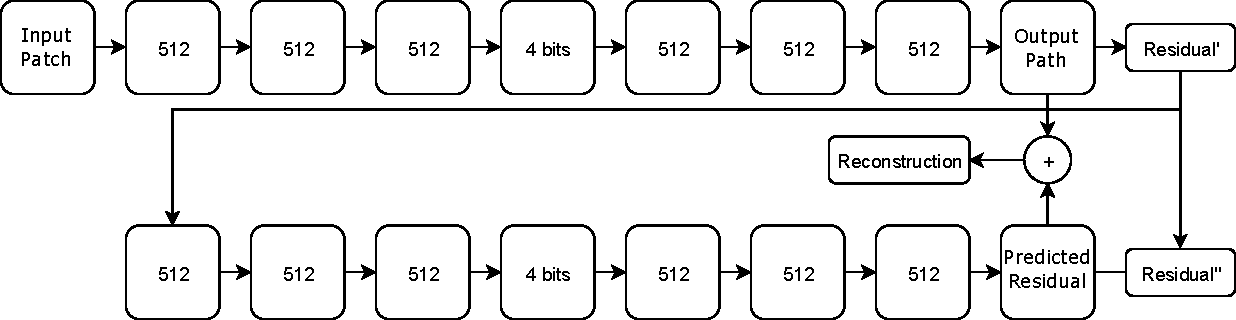
\includegraphics[width=0.90\textwidth]{figuras/toderici_1.pdf}
	\caption[Autocodificador residual totalmente conectado.]{Um autocodificador residual totalmente conectado com  função de ativação $\tanh$. Esta figura representa uma arquitetura de duas iterações. As primeiras iterações codificam a imagem original. Os resíduos da reconstrução são passados para a segunda iteração. Cada nível de iteração produz 4 bits \cite{Variable2016Toderici}.}
	\label{fig:toderici1}
\end{figure}


Os autores estenderam essa arquitetura substituindo as camadas totalmente conectadas pelos operadores de convolução no codificador $E$ e pelos operadores ``deconvolucionais'' ou de convolução transposta no decodificador $D$ \cite{Variable2016Toderici}.

%Consulte \cite{Variable2016Toderici} para obter a formulação matemática da convolução transposta.Pela própria definição da \acrshort{conv2d} a taxa gerada na binarização é independente do tamanho da imagem de entrada. Os autores definiram essa taxa a 2 bits por pixel por iteração. A figura \ref{fig:toderici2} mostra essa arquitetura (exceto a conversão RGB). 


%\begin{figure}[h]
%	\centering
%	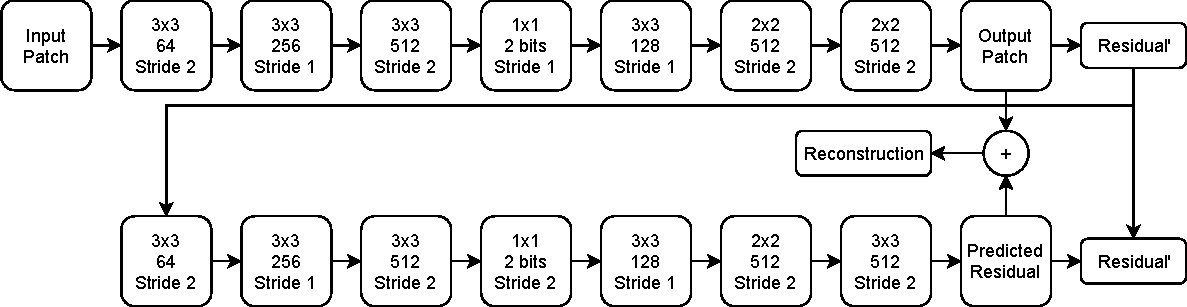
\includegraphics[width=0.90\textwidth]{figuras/toderici_2.pdf}
%	\caption{O codificador residual convolucional/deconvolucional. As camadas
%		convolucionais são representadas como retângulos pontiagudos, enquanto as
%		camadas deconvolucionais são representadas como retângulos arredondados. \cite{Variable2016Toderici}.}
%	\label{fig:toderici2}
%\end{figure}

\subsection{Redes Recorrentes}

%Muitas implementações de camadas foram propostas para manter a informação temporal. Uma das primeiras abordagens eficazes baseiam-se na Long Short-Term Memory (LSTM). Aprimoramentos posteriores incluem a Unidade Recorrente Gated (GRU), que simplifica o componente recorrente ao mesmo tempo em que obtém desempenho similar ao \acrshort{lstm} em alguns cenários \cite{NeuralReview2019Siwei}.


Em autocodificadores recorrentes podemos incluir a memória da rede para capturar as dependências entre os resíduos gerados em cada iteração. Além disso, essa característica permite ao modelo  estimar diretamente a imagem original em cada estágio $t$, isto é, $F_t$($r_{t-1}$) = $x'_{t}$ ou obter a reconstrução dos resíduos por iteração como apresentado na Equação \ref{eq:reconst_escalar}. 
Nessas abordagens, o encadeamento de autocodificadores é implícito (uso recursivo do autocodificador). Outra motivação de usar camadas recorrentes é a redução no número de parâmetros do modelo a serem aprendidos. 

Ainda no trabalho \cite{Variable2016Toderici}, explorou-se o uso de modelos recorrentes em duas arquiteturas. Na primeira, o codificador é composto por uma camada totalmente conectada seguida por duas camadas \acrshort{lstm} empilhadas. O decodificador tem a estrutura oposta: duas camadas \acrshort{lstm} empilhadas seguidas por uma camada totalmente conectada com uma não-linearidade que prediz os valores RGB. Aqui, o modelo da \acrshort{lstm} segue a formulação da Equação \ref{eq:lstm}.

A Figura \ref{fig:toderici_ae_lstm} mostra um desenrolar dessa rede com camadas \acrshort{lstm} (menos a conversão RGB), necessária para o treinamento, em duas etapas de tempo. As conexões verticais entre os estágios \acrshort{lstm} no mostram o efeito de propagação de memória. 
Na segunda abordagem, os autores combinam os operadores convolucionais e deconvolucionais com a \acrshort{lstm}. Tal arquitetura obteve a melhor performance dentre os testes realizados. %Entraremos em detalhes dessa formulação.  


\begin{figure}[h]
	\centering
	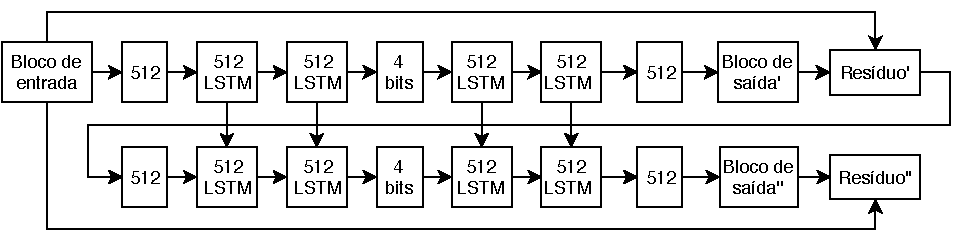
\includegraphics[width=0.90\textwidth]{figuras/ae_lstm.pdf}
	\caption[Autocodificador residual com camadas \acrshort{lstm}]{ Esta figura mostra o autocodificador com camadas  \acrshort{lstm}em duas iterações de treinamento.  Ao todo, a rede foi treinada com 16 níveis de resíduo, para gerar representações de 64 bits. As conexões verticais entre os estágios \acrshort{lstm} no desenrolamento mostram o efeito da memória persistente. Nessa arquitetura \acrshort{lstm}, cada etapa prevê a saída real. \cite{Variable2016Toderici}.}
	\label{fig:toderici_ae_lstm}
\end{figure}

%Nesse trabalho, os autores usaram um banco de dados de referência com 
%216 milhões de imagens coloridas e coletadas aleatoriamente da internet. Essas imagem foram reduzidas para blocos de $32 \times 32$ que elimina artefatos de compactação preexistentes para a maioria das imagens \cite{Variable2016Toderici}. Para o treinamento dos modelos \acrshort{lstm}, 90\% das imagens foram utilizadas; os restantes 10\% foram reservados para avaliação.  

A função de custo utilizada foi a métrica $L_2$ nos resíduos. Ela é definida substituindo $p=2$ na Equação a seguir \cite{nie2010efficient}:
\begin{equation}
||v||_p = \left ( \sum_{i=1}^n |v_i|^p \right)^{\frac{1}{p}}  
\end{equation}

onde, $v \in \mathbb{R}^n$ é um vetor sobre o qual estamos aplicando a norma $L-p$. 



%Uma rede neural recorrente RNR é um tipo de rede neural com memória para armazenar informações sobre entradas passadas. 
%Uma unidade recorrentes são úteis para processamento de sequências em que a predição atual depende de informações passada. Para que isso seja possível, essa unidades possui uma estrutura em cadeia de modo que sua saída anterior $h_{t-1}$  é usada como parte da entrada no novo processamento - são conexões consigo mesmas. 




%A camada \acrshort{lstm} possui a seguinte formulação, em que $ x_t $, $ c_t $ e $ h_t $ indicam os estados de entrada, célula e ocultos na iteração $ t $ \ citeC{FullResolution2017Toderici}:

%\begin{equation}
%	\begin{aligned}
%	{[f, i, o, j]}^T & = [\sigma, \sigma, \sigma, \tanh]^T((Wx_t + Uh_{t-1}) + b) \\
%	c_t & = f \odot c_{t-1} + i \odot j \\
%	h_t & = o \odot \tanh(c_t)
%	\end{aligned}
%\end{equation}
%onde $\odot $ é a multiplicação de elementos, $b$ é o bias e $\sigma$ é a função sigmóide. A saída da camada é $h_t$. 


%Duas arquiteturas propostas em \cite{Variable2016Toderici} utilizam a abordagem recorrente. Na primeira arquitetura, E e D consistem de camadas \acrshort{lstm} empilhadas além de camadas totalmente conectadas. A figura em mostra um desenrolar do \acrshort{lstm}, necessário para treinamento, em duas etapas de tempo. As conexões verticais entre os estágios \acrshort{lstm} no desenrolar mostram o efeito de propagação de memória. 
%Observe que, em contraste com a Figura 1, em que a rede após a primeira etapa é usada para prever o erro residual da etapa anterior, nessa arquitetura \acrshort{lstm}, cada etapa prevê a saída real.

%Na segunda abordagem os autores combinam os operadores convolucionais e desconvolucionais com o \acrshort{lstm}. Definiu-se o \acrshort{lstm} convolucional substituindo a transformação Tl 4n na equação (8) por convoluções mais vieses. Então a função de transformação para \acrshort{lstm} convolucional com passo k é
%Aqui usamos os índices c e d para diferenciar os pesos associados às operações de convolução e deconvolução. Para construir o decodificador deconvolucional de \acrshort{lstm}, substituímos a segunda e terceira camadas deconvolucionais do decodiftexicador deconvolucional da Figura 3 por \acrshort{lstm} deconvolucional.

Em \cite{FullResolution2017Toderici} foi proposto um modelo convolucional-recorrente como resultado de melhorias do trabalho em \cite {Variable2016Toderici}. A ideia central permanece a mesma: encadeamento de autocodificadores treinados sobre os resíduos e com taxa de compressão fixa por iteração.  Tal arquitetura é representada compactamente através da Equação \ref{eq:ae_full}. 

\begin{equation}
\label{eq:ae_full}
\begin{aligned}
r_{0} &=x\\
b_{t} &= B(E_{t}(r_{t-1})) \\
\hat{x}_{t} &= D_{t}(b_{t}) + \gamma \hat{x}_{t-1} \\
r_{t} &= x- \hat{x}_{t}
\end{aligned}
\end{equation}

onde $E_t$, $D_t$, $b_t$, $\hat{x}_t$ e $r_t$ representam, respectivamente, codificador, decodificador, fluxo de bits, reconstrução progressiva da imagem original $x$, e o residual entre $x$ e $\hat{x}_t$ na iteração $t$. Se o valor de $\gamma$ é zero a reconstrução é do tipo única (``um disparo''), caso contrário, $\gamma = 1$ , e teremos a reconstrução aditiva. Na reconstrução única cada iteração sucessiva tem acesso a mais bits gerados pelo codificador, o que permite uma melhor reconstrução. 

%Em cada iteração, a função $B$ produzirá $m$ bits pertencente ao conjunto ${-1,1}^m$.  Após k iterações, a rede produz $m x k$ bits no total.  m é uma função linear do tamanho da entrada. Para patches de imagem de 32x32, m = 128.

O modelo é composto por camadas \acrshort{conv2d}; hibridas do tipo convolucional-recorrente (\acrshort{conv2drnr}); e camadas estáticas de binarização e de \gls{pe}. A figura \ref{fig:toderici3} apresenta um fluxograma da arquitetura para uma iteração. 





As camadas \acrshort{conv2drnr} seguem formulação matemática dependente do tipo de rede recorrente.  Nela temos 4 camadas no : 3 convolucionais e 1 RNN-Conv; 1 camada de binarização do tipo convolucional; e 6 camadas no enconder: 2 convolucionais e 4 unidades RNN-Conv
Em um dos modelos, os autores empregam a \acrshort{conv2dlstm} descrita pela Equação \ref{eq:conlstm}. Também foram testadas a \acrshort{lstm} associativa e a \gls{gru}.
Independentemente da camada recorrente, dentre as 3 citadas, as \acrshort{conv2drnr} incluem duas convoluções 2D: uma no vetor de entrada, $x_t$, outra no vetor de estado oculto anterior, $h_{t-1}$, que será referida como ``convolução oculta'' realizada pelo  ``filtro oculto''. Os resultados das convoluções são somados e seguem para uma etapa de processamento (dependente da rede recorrente) para fornecer $h_t$ e $c_t$.

A \acrshort{pe} interpola os \textit{pixels} em diferentes canais para formar imagens de alta resolução de acordo com fator de escala, $upscale\_factor$. Essa operação também é conhecida como \textit{PixelShuffle}. Para exemplificar, seja uma entrada $X$ e fator de escala $uf$, então obteremos a saída $Y$ segundo:   

\begin{equation}
\label{eq:pf}
\begin{aligned}
dim(X) &= (N,L,H_{in}, W_{in}) \\
L &=  C \times \text{uf}^2 \\ 
Y &= pixel\_shuffle(X, \text{uf}) \\
dim(Y) &= (N,C,H_{in} \times \text{uf}, W_{in}\times \text{uf}) 
\end{aligned}
\end{equation} 

onde $dim \left( \odot \right)$ retornar a dimensão de um tensor. A \acrshort{pe} reduz o número de canais e aumenta a dimensão espacial, por isso pode ser usada em substituição a convolução transposta.  

\begin{figure}[h]
	\centering
	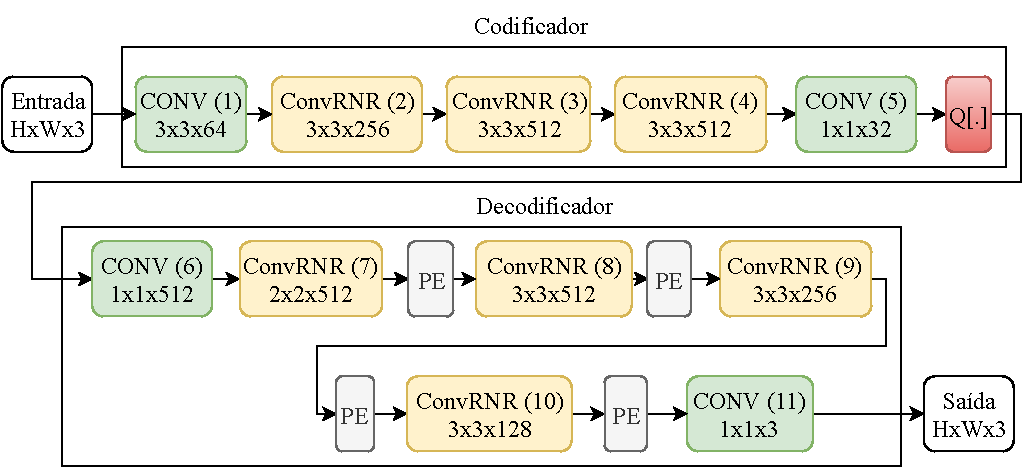
\includegraphics[width=1.00\textwidth]{figuras/toderici_3.pdf}
	\caption[Arquitetura do autocodificador com camadas Con2DRNR]{ Esta Figura mostra a arquitetura de um autocodificador com camadas recorrentes  e convolucionais para compressão de imagens de alta resolução. Nas camadas convolucionais, em verde, está indicada o formato do seu filtro convolucional (altura x largura x número de canais). Para cada camada ConvRNR o formato de filtro mostrado contém as dimensões  espaciais dos núcleos aplicados no tensor de entrada e o número de filtros desses núcleos e dos núcleos ocultos. As dimensões espaciais dos filtros ocultos nas ConvRNR são todas 1x1, exceto as camadas 9 e 10 onde são 3x3. Em vermelho está indicado a função de binarização.  As camadas de profundidade para espaço reduzem por um fator de 4 o número de canais do tensor de entrada e aumenta cada dimensão espacial por um fator de 2. Todas as operações de convolução são bidimensionais. Figura adaptada de \cite{FullResolution2017Toderici}}.
	
	\label{fig:toderici3}
\end{figure}

%Existem algumas diferenças de arquitetura, embora sejam semelhantes em um contexto geral.


Durante o treinamento dos modelos em \cite{FullResolution2017Toderici} uma perda ponderada de $L_1$ é calculada sobre os resíduos gerados em cada iteração, isto é, a perda total é $\beta \sum_t|r_t|$. Apenas ao final das iterações de recorrência é que ocorre a atualização dos pesos. A partir desse ponto diversas melhorias foram propostas na tentativa de contornar limitações impostas pelo modelo.

%Para treinar o modelo foram usados dois conjuntos de imagens de $32 \times 32 \times 3$. O primeiro corresponde a base de dados usados em \cite{Variable2016Toderici}.
%Para obter o segundo conjunto de dados, primeiro reuniu-se uma amostra aleatória de 6 milhões de imagens de $1280 \times 720$ da \textit{Web} que foram decompostas em blocos em $32 \times 32 \times 3$ sem sobreposição  e codificadas com PNG. Então os 100 blocos de mais alta entropia por imagem, isto é, com a pior taxa de compactação, foram novamente amostrados e reunidos no segundo conjunto de dados. 

%O fluxo da informção usando essa rede de ganho é mostrado na Figura \ref{fig:toderici4}.
Ainda, em \cite{FullResolution2017Toderici} os autores usam uma rede neural específica, $G$,  para promover um fator de ganho nos resíduos. A saída dela é condicionada pela reconstrução e iteração, isto é, $g_t = G(x'_t)$. A intenção é impedir que o erro residual se torne ínfimo a ponto de comprometer a convergência do modelo. 
Outra melhoria proposta foi a adição de uma nova \acrshort{rna} de codificação de entropia para melhorar a taxa de compactação. De forma simplificada, é empregado uma rede recorrente binária, baseada em uma \acrshort{lstm}, que induz um modelo de probabilidade a um codificador aritmético.





%Uma das principais desvantagens das propostas de ponta a ponta é a não flexibilidade das redes, como mencionado anteriormente. Essa rigidez impõe uma restrição na variabilidade do número de bits aplicado a cada patch. \cite{FullResolution2017Toderici} também tenta resolver esse problema pelo menos no contexto da codificação de entropia. 

%Assim, os autores propõem uma rede recorrente binária, baseada em um \acrshort{lstm}, que induz um modelo de probabilidade a um codificador aritmético. A figura \ref{fig:toderici5} representa a modelagem referida

%\begin{figure}
%	\centering
%	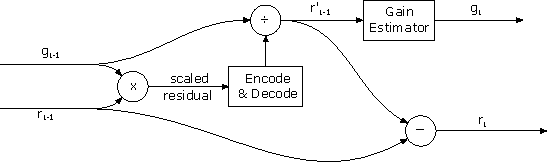
\includegraphics[width=0.90\textwidth]{figuras/toderici_4.pdf}
%	\caption{Using a content-dependent residual to the framework. This scalar gain factor is applied to all color channels \cite{FullResolution2017Toderici}.}
%	\label{fig:toderici4}
%\end{figure}

%Essa arquitetura é baseada no PixelRNN e usa uma linha de estados $S$ de tamanho $1 \times W \times k$ para capturar dependências de curto e longo prazo para modelar probabilidades de código. Uma convolução mascarada de $7 \times 7$ é aplicada e produz um $z_0$. Este \acrshort{lstm} processa uma linha de varredura por vez. A última etapa é composta de convoluções de $1 \times 1$ para aumentar a capacidade de memorização da rede.

%\begin{figure}
%	\centering
%	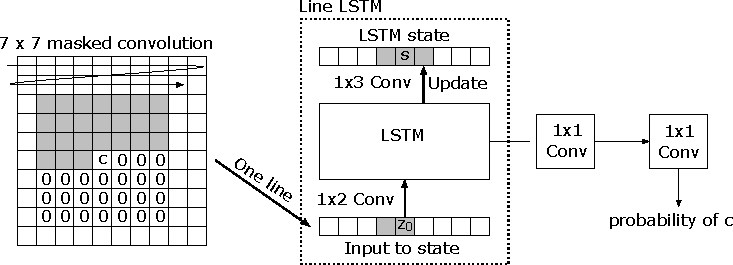
\includegraphics[width=0.70\textwidth]{figuras/toderici_5.pdf}
%	\caption{BinaryRNN \cite{FullResolution2017Toderici}.}
%	\label{fig:toderici5}
%\end{figure}

%A arquitetura ponta a ponta apresenta a vantagem de controle na taxa de bits que está relacionado com o gargalo da rede. As reconstruções progressivas são obtidas em virtude do uso da informação residual. Contudo, ela apresenta as seguintes desvantagens:

%\begin{itemize}
%    \item Consumo de muito recurso computacional 
%    \item Tempo para codificar e decodificar uma imagem em modelo treinadao
%    \item Uso do mesmo número de bits para comprimir patches simples (baixa entropia) e complexos (alta entropia)   
%    \item Rigidez para controlar a qualidade da imagem através de alguma métrica alvo 
%\end{itemize}


%O treinamento foi realizado com o otimizador Adam com taxas de aprendizado de $\{0.1, 0.3, 0.5, 0.8, 1\}$ e uma perda normalizada de $ L_2 $. O número de iterações variou de 8 a 16. O \acrshort{ssim} é usado para avaliar o desempenho em tempo de teste. Vale a pena notar que esta solução introduz artefatos de codificação em limites de patch.


%Em trabalhos posteriores houve atenção especial para otimizar o modelo apresentado em \ref{fig:toderici3}. 

Em \cite{target} os autores modificaram a rede \ref{fig:toderici3} 
para usar 0/1, em vez de -1/1 a fim de evitar artefatos de limite nas bordas das imagens. Além disso, eles implementaram um método para que a rede possa alocar mais bits nos blocos mais difíceis de reconstruir em comparação com os mais simples. 
Para que isso fosse possível uma camada com máscara é utilizada sobre o código binário gerado e aplicado após a primeira iteração da rede, no tempo de treinamento.
O mascaramento pode ser transparente sobre esse código binário e, nesse caso, a saída dessa camada coincide com o código binário. Contudo, se em uma dada iteração da rede pelo menos uma das seguintes condições forem satisfeitas, a máscara levará todos os bits para zero. 

\begin{itemize}
	\item  Onde a qualidade de reconstrução do bloco excede o nível de qualidade desejado;
	\item A saída do codificador é acidentalmente zero;
	\item Os códigos foram mascarados em uma iteração anterior.
\end{itemize}

Essa lógica de mascaramento permite tratar um código de bits zero como um sinal de parada e evitar o envio de qualquer informação subsequente do codificador para o decodificador.  Neste trabalho, outra mudança atingiu a função de perdas da rede. Para essa função, foi considerada a perda $L_1$ sobre os resíduos (erro de reconstrução) e uma função (não detalhada no referido artigo) proporcional a quantidade de bits diferente de zero. O propósito dessa segunda parcela  é tornar o código binário com maior taxa de 0 e possibilitar compactação de entropia mais eficaz. A codificação de entropia usada foi a LempelZiv (LZ77). 
Os \acrshort{codec}'s de imagens que apresentam melhor desempenho se valem do conteúdo espacial da imagem para alocar os bits disponíveis de forma otimizada. Tal técnica é empregada, por exemplo, pelo JPEG2000, WebP e \acrshort{bpg} \cite{boliek2000information}. No trabalho apresentado por Minnen et. al. em \cite{SpatiallyAdaptive2018Minnen} é discutido um método para implementar uma alocação de bits com base na complexidade de regiões de imagens. Na prática, essa adaptação da taxa se dá pela correlação entre os blocos próximos de uma imagem. 

%Aqui, essa tarefa ocorrerá em tempo de treinamento para promover adaptação na taxa de bits com base na . 

Aqui, o \acrshort{codec} proposto é composto por duas redes neurais para realizar tarefas específicas. A primeira rede deverá gerar previsões de blocos da imagem a partir dos blocos vizinhos, a segunda recebe o resíduo dessa previsão para reconstruí-lo progressivamente. 
Ao final, a reconstrução da imagem corresponde a primeira previsão somada aos resíduos reconstruídos. A primeira rede é um autocodificador convolucional, ilustrado na Figura \ref{fig:toderici8}, que recebe 1 bloco $64 \times 64$ ou, de forma equivalente, 4 blocos $32 \times 32$, sendo 3 deles da imagem original e um bloco com pixels zeros. Este último é o alvo que a rede tentará prever na saída ao minimizar o erro $L_1$ entre essa previsão e o bloco original.  A figura \ref{fig:toderici7} ilustra o processo de previsão descrito.     


\begin{figure}
	\centering
	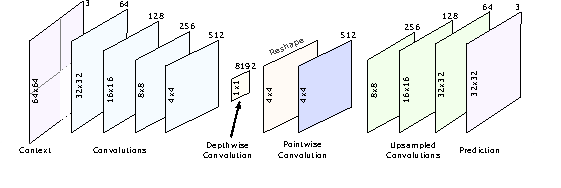
\includegraphics[width=0.90\textwidth]{figuras/toderici_8.pdf}
	\caption[Modelo DPCM com autocodificador.]{A rede de previsão com base no contexto espacial é um codificador automático que recebe uma imagem de $64 \times 64$, com zeros no bloco atual e gera esse bloco ausente\cite{SpatiallyAdaptive2018Minnen}.}
	\label{fig:toderici8}
\end{figure}

\begin{figure}
	\centering
	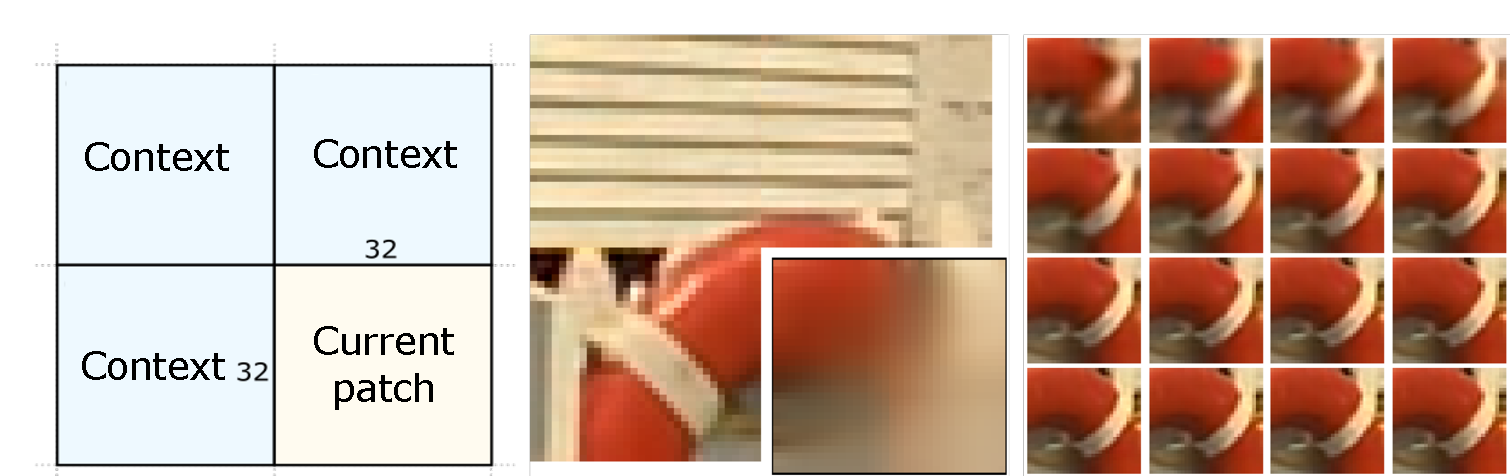
\includegraphics[width=0.90\textwidth]{figuras/toderici_7.pdf}
	\caption[]{Para cada  $32 \times 32$, o modelo DPCM tenta prever com base nos blocos vizinhos. Os resíduos são propagados para o autocodificador \cite{SpatiallyAdaptive2018Minnen}.}
	\label{fig:toderici7}
\end{figure}

A segunda rede, irá complementar a tarefa da primeira ao reconstruir a informação residual. Ela corresponde a rede \ref{fig:toderici3} com reconstrução aditiva e usando unidades Con2DLSTM. 

%“LSTM (Additive Reconstruction)” apresentada por Toderici et al. [2], exceto que onde esse papel treina a rede para compactar imagens completas, treinamos para compactar o resíduo em cada bloco após executar o preditor de contexto.


No artigo \cite{Priming2017Johnston}, Johnston et al. implementaram 3 modificações na forma de treinar o modelo que o fez superar os \acrshort{codec}'s \acrshort{bpg}(4:2:0), WebP, JPEG2000 e \acrshort{jpeg} medidos na métrica \acrshort{msssim}. 

A primeira mudança foi na execução de iterações falsas na rede (passos adicionais) a fim de inicializar os estados ocultos das camadas recorrentes ($h_t$ e $c_t$) com valor diferente de zero - essa técnica foi chamada de \textit{k-priming} de estado oculto.
Nessa técnica, um lote de imagens passa k vezes pela rede do codificador descartando os bits gerados nas primeiras k-1 vezes (falsas iterações). Todavia as alterações nos tensores de estado oculto das unidades recorrentes do codificador são mantidas. Quando o lote passa pela k-ésima vez pelo codificador teremos uma iteração real e os bits são transmitidos para o decodificador. 
De forma análoga, na rede do decodificador esses bits são usados para reconstruir k vezes o conjunto de imagens. Dessa forma, a rede consegue inicializar os estados ocultos do decodificador e na iteração k a reconstrução será válida para continuar o treinamento.    

O \textit{k-priming} pode ser executado, também, entre as iterações e é especificamente denominado por \textit{k-difusão}. Essa técnicas proporcionaram melhores resultados, mas ao custo de exigir mais tempo de execução e recursos computacionais \cite{Priming2017Johnston}. 

%Tanto no \textit{k-priming} quando na \textit{k-difisão}  à medida que aumentamos k, aumentamos o suporte máximo do sistema junto com o tempo de computação e treinamento.
%Por exemplo, para representar regiões da imagens de baixa frequência (por exemplo o céu sem nuvens) são necessários menos bits que informações de alta frequência (por exemplos confetes).

Como foi discutido a abordagem de redes neurais em cascata adiciona uma quantidade fixa de bits em cada iteração. Esse fato torna a rede ineficiente na medida que, independentemente da complexidade da imagem, o mesmo número de bits são utilizados para representá-la.  A solução proposta pelos autores em \cite{Priming2017Johnston} é, dada uma qualidade de destino, atribuir a cada bloco de $16 \times 16$ pixels uma quantidade de bits suficientes para atender ou exceder a qualidade de destino até o máximo suportado pelo modelo.
Esse processo ocorre no tempo de teste da rede (após o seu treinamento) e algumas  heurísticas foram adotadas para evitar artefatos de compressão. O bloco pode ser subdividido em 4 blocos  $8 \times 8$, sobre os quais obtém-se a norma $L_1$ do erro residual. A qualidade do bloco $16 \times 16$ será tomado como o valor máximo dentre as 4 medidas de erro. Cada bloco $16 \times 16$ usará entre $50\%$ e $120\%$ da taxa de bits de destino (arredondado para a iteração mais próxima). 
O codificador terá que criar uma matriz para indicar quantos bits foram reservados para cada localização da imagem. O algoritmo do decodificador requer que todos os bits estejam presentes para reconstruir uma imagem, logo ele preenche com um valor numérico as regiões nas quais o codificador reservou menos bits que o máximo possível. O valor adotado pelos autores foi 0, o valor médio da binarização (-1 e 1). 
Por fim, a terceira mudança recaiu na função de custo. Os autores adotaram uma função para considerar, além do erro tradicional de $L_1$, uma métrica perceptual de qualidade. Ela corresponde a métrica $L1$ ponderada por uma função que mede a dissimilaridade perceptual entre duas imagens \ref{eq:loss}.    

\begin{equation}
\label{eq:loss}     
\begin{aligned}
L(x,x') &= w(x,x') \times L_1(x-x') \\ 
w(x,x') &= \frac{S(x,x')}{\bar{S}} 
\end{aligned}
\end{equation}

onde $S(x, x')$ é uma medida perceptual da dissimilaridade entre as imagens $x$ e $x'$ e  $\bar{S}$ é ajustada para a média móvel de $S(x,x')$. 
Intuitivamente, essa perda está realizando amostragem de importância dinâmica: compara a distorção perceptual de uma imagem com a distorção perceptiva média e pesa mais as imagens com alta distorção perceptual e menos pesadamente as imagens para as quais a rede de compressão já funciona bem.
Na prática, $S(x, x')$ foi modela pela medida de dissimilaridade $D(x, x') = 0,5 \times (1- \acrshort{ssim} (x, x'))$. 
A Tabela \ref{table:codecs} apresenta as principais características dos autocodificadores em cadeia, relatos neste trabalho.  

%Na prática, a imagem é dividida em blocos $8 \times 8$. Para cada bloco é calculado um valor de ponderação local, dado pela dissimilaridade: $D(x, x') = 0,5 \times (1- \acrshort{ssim} (x, x'))$. A perda em toda a imagem, $L(x,x')$, é igual a soma de $D(x,x')$ ponderadas localmente por $L_1$.


\begin{landscape}
	
	\begin{table}[htbp]
		\caption[Tabela com resumo de \acrshort{codec}'s baseados em autocodificadores em cadeia.]{Tabela com informações sintetizadas do \acrshort{codec}'s de imagens baseados em autocodificadores em cadeia.}
		\begin{adjustbox}{width=\columnwidth,center}
			\begin{tabular}{|l|l|l|l|l|l|}
				\hline
				\rowcolor[HTML]{EFEFEF} 
				\multicolumn{1}{|c|}{\cellcolor[HTML]{EFEFEF}Autores}  & \multicolumn{1}{c|}{\cellcolor[HTML]{EFEFEF}Autocodificador}                                                                                                                 & \multicolumn{1}{c|}{\cellcolor[HTML]{EFEFEF}Descrição}                                                                                                                                                                                         & \multicolumn{1}{c|}{\cellcolor[HTML]{EFEFEF}
					\begin{tabular}[c]{@{}c@{}}Função de custo e\\ Base de treinamento\end{tabular}}
				& \multicolumn{1}{c|}{\cellcolor[HTML]{EFEFEF}\begin{tabular}[c]{@{}c@{}}	Controle de\\ taxa e /ou qualidade \end{tabular}}                                                                                                                                    & \multicolumn{1}{c|}{\cellcolor[HTML]{EFEFEF}\begin{tabular}[c]{@{}c@{}}Comparação com\\  \acrshort{codec}'s tradicionais\end{tabular}}                                                                           \\ \hline
				Toderici et. al.  \cite{Variable2016Toderici}       & \begin{tabular}[c]{@{}l@{}}- Totalmente conectado \\ - Recorrente \\ - Convolucional \\ - Convolucional \acrshort{lstm}\\ - Encadeamento implícito \\ ou explícito  de ACs\end{tabular} & \begin{tabular}[c]{@{}l@{}}- Modelo opera sobre os \\ resíduos  em  16 iterações \\  - Reconstrução aditiva ou \\ única\end{tabular}                                                                                                           & \begin{tabular}[c]{@{}l@{}}- Norma $L_2$ aplicada nos resíduos\\ - Base com 216 milhões de imagens\\  obtidas da internet e subamostradas \\ para blocos $32 \times 32$\end{tabular}                                           & \begin{tabular}[c]{@{}l@{}}- Controle da taxa é\\ feito pelo número de \\ iterações na reconstrução\\ dos blocos.\end{tabular}                                                                                                                              & \begin{tabular}[c]{@{}l@{}}- O modelo convolucional\\  \acrshort{lstm}  supera  o \acrshort{jpeg} \\ em \acrshort{ssim}  dentro do \\ intervalo 0,125 a 1,375 bpp.\end{tabular}                                                       \\ \hline
				Toderici et. al.  \cite{FullResolution2017Toderici} & \begin{tabular}[c]{@{}l@{}}- Convolucional \acrshort{lstm} \\ - Convolucional \acrshort{lstm}\\ associativa\\ - Convolucional GRU\\ - Encadeamento implícito\end{tabular}                          & \begin{tabular}[c]{@{}l@{}}- Modelo opera sobre os \\ resíduos  em  16 iterações\\ - Reconstrução aditiva ou \\ única\\ - \acrshort{rna} para camada de \\ fator de ganho dos resíduos\\ - \acrshort{rna} para gerar contexto\\ de codificação aritmética\end{tabular} & \begin{tabular}[c]{@{}l@{}}- Norma $L_1$ aplicada nos resíduos\\ - Base reunida em \cite{Variable2016Toderici} e um novo\\ conjunto de blocos $32 \times 32$ de alta\\ entropia recortados de 6 milhões\\ de imagens $1280 \times 720\textbf{}$ que foram\\ coletadas aleatoriamente da internet	
				\end{tabular}                                           & \begin{tabular}[c]{@{}l@{}}- Controle da taxa é\\ feito pelo número de \\ iterações na reconstrução\\ dos blocos\\ - Codificação de entropia\\ reduz a taxa\end{tabular}                                                                                    & \begin{tabular}[c]{@{}l@{}}- O modelo Convolucional\\  GRU  de reconstrução \\ única supera o \acrshort{jpeg} \\ em  \acrshort{msssim} e \acrshort{psnr}-HVS\\ dentro  do intervalo 0,1 a 1,5 \\  bpp (aproximadamente)\end{tabular} \\ \hline
				Covell et. al.  \cite{target}                       & \begin{tabular}[c]{@{}l@{}}- Convolucional \acrshort{lstm}\\ - Encadeamento implícito\end{tabular}                                                                                      & \begin{tabular}[c]{@{}l@{}}- Modelo opera sobre os \\ resíduos  em  16 iterações.\\ -  Reconstrução aditiva \\ com ganho residual\\ - Implementação de \\ códigos de parada\\  - LZ77 é usado para \\ codificação de entropia\end{tabular}     & \begin{tabular}[c]{@{}l@{}}- Norma $L_1$ aplicada nos resíduos \\ e penalidade pela ocorrência de \\bits diferentes de zero\\ - Base de treinamento formada por \\blocos $32 \times 32$\end{tabular} & \begin{tabular}[c]{@{}l@{}}- Controle da taxa é\\ feito pelo número de \\ iterações na reconstrução\\ dos blocos\\ - A qualidade alvo é \\ usada  para  adaptar  as\\  taxas  de bits por\\  blocos\\ - Codificação de entropia\\ reduz a taxa\end{tabular} & \begin{tabular}[c]{@{}l@{}}- O modelo supera o \acrshort{jpeg} em \\ \acrshort{psnr} dentro  do intervalo \\ 0.125 a 1,375 bpp\\  (aproximadamente)\end{tabular}                                                           \\ \hline
				Minnen et. al.  \cite{SpatiallyAdaptive2018Minnen}  & \begin{tabular}[c]{@{}l@{}}- Convolucional \acrshort{lstm}\\ - Encadeamento implícito\end{tabular}                                                                                      & \begin{tabular}[c]{@{}l@{}}- Modelo opera sobre os \\ resíduos  em  16 iterações.\\ - AC para  predição de  \\ contexto\\ - Reconstrução aditiva\end{tabular}                                                                                  & \begin{tabular}[c]{@{}l@{}}- AC de contexto: norma $L_1$ \\ sobre o resíduo\\ - AC \acrshort{conv2dlstm}: função de \\custo não especificada \\- Base de treinamento composta\\ por blocos $64 \times 64$ de alta entropia\\ recortados de 6 milhões de imagens\\ $1280 \times 720$,  seguindo método em \cite{FullResolution2017Toderici}   \end{tabular} & \begin{tabular}[c]{@{}l@{}}- Controle da taxa é\\ feito pelo número de \\ iterações na reconstrução\\ dos blocos\end{tabular}                                                                                                                               & \begin{tabular}[c]{@{}l@{}}- O modelo supera o JPEG\\  em \acrshort{psnr}  dentro do \\ inverva-lo de 0,25 a 1,5 bpp\end{tabular}                                                                               \\ \hline
				Jonhston et. al.  \cite{Priming2017Johnston}        & \begin{tabular}[c]{@{}l@{}}- Convolucional \acrshort{lstm}\\ - Encadeamento implícito\end{tabular}                                                                                      & \begin{tabular}[c]{@{}l@{}}- Codificação com uma\\  arquitetura de \\ 16 iterações que memória.\\  - iterações falsas\\  - Método de alocação de\\ bits pós treinamento\end{tabular}                                                           & \begin{tabular}[c]{@{}l@{}}- Norma $L_1$ sobre os resíduos  \\ponderada pela DSSIM \\
					- Base de treinamento é formada \\por blocos $128 \times 128$ amostrados \\aleatoriamente de 6 milhões de\\ imagens $1280 \times 720$ da internet
					
				\end{tabular}                        & \begin{tabular}[c]{@{}l@{}}- Controle da taxa é\\ feito pelo número de \\ iterações na reconstrução\\ dos blocos\\  - A qualidade alvo é \\ usada  para  adaptar  as\\  taxas  de bits por blocos\end{tabular}                                              & \begin{tabular}[c]{@{}l@{}}O modelo supera o BPG\\  no \acrshort{msssim} dentro do \\ intervalo 0,125 a 2  bpp \\ (aproximadamente)\end{tabular}                                                               \\ \hline
			\end{tabular}\quad
		\end{adjustbox}
		\label{table:codecs}
	\end{table}
\end{landscape}

%\end{landscape}

\section{Autocodificadores variacionais}



Diferentemente dos autocodificadores que produzem diretamente $z$ no gargalo, os VAE produzem duas matrizes, representando média e variância, para caracterizar os gaussianos. Essa matriz representa o $P(z)$ (PDF da variável latente $z$) e é feita uma amostragem. Portanto, o codificador e o decodificador são as funções usadas para induzir a distribuição e mapear os gaussianos fatorados para a distribuição real, reconstruindo a amostra \cite{DeliverableSeptember}. 
O autocodificador variacional foi empregado em  \cite{End2016Balle} na tarefa de compressão de imagens ao tentar modelar taxa e distorção, $R +\lambda D$. Os autores desenvolveram uma estrutura para otimização de ponta a ponta de um modelo de compressão de imagem baseado em transformações não-lineares.
Eles usaram um módulo de não-linearidade denominado: normalização divisiva generalizada (GDN) que se mostrou eficaz na gaussianização de densidades de imagem. 
Para qualquer ponto desejado ao longo da curva de taxa-distorção, os parâmetros das transformações de análise e síntese do modelo são otimizados em conjunto.
Para conseguir isso na presença de quantização, os autores usam  um relaxamento contínuo do modelo de probabilidade, e substituem a etapa de quantização por ruído uniforme aditivo. 

%Finalmente, em vez de relatar estimativas de entropia diferencial ou discreta, implementamos um código de entropia e relatamos o desempenho usando taxas de bits reais, demonstrando assim a viabilidade de nossa solução como um método completo de compactação com perdas.
Esse trabalho foi aprimorada em  \cite{Variational2018Balle,Autoregressive2018Minnen}. Entre as inovações, destaca-se modelo autoregressivo através de redes neurais \cite{Autoregressive2018Minnen} e  distribuição anterior em um hiperparâmetro \cite{Autoregressive2018Minnen,Variational2018Balle}. Duas desvantagens da abordagem usando  \acrshort{vae} para compressão de imagens, presentes nesses trabalhos, são a necessidade de treinar muitos modelos e exigência muito recurso computacional no treinamento. 

%A transformação de análise $g_a$ consiste em três estágios de convolução, subamostragem e normalização divisiva. Analogamente, a transformada de síntese $g_s$ consiste em três estágios, com a ordem das operações invertida dentro de cada estágio: IGDN (inverso aproximado da GDN), superamostragem e convolução.

%Esta transformação é seguida por quantização escalar uniforme (isto é, cada elemento é arredondado para o número inteiro mais próximo), o que implementa efetivamente uma forma paramétrica de quantização vetorial no espaço da imagem original. 
%A imagem comprimida é reconstruída a partir destes valores quantificados usando uma transformação inversa não linear paramétrica aproximada.

%Para qualquer ponto desejado ao longo da curva de taxa-distorção, os parâmetros de ambas as transformações de análise e síntese são otimizados em conjunto usando a descida de gradiente estocástica. Para conseguir isso na presença de quantização (que produz zero gradientes em quase todos os lugares), usamos uma função de perda de proxy baseada em um relaxamento contínuo do modelo de probabilidade, substituindo a etapa de quantização por ruído uniforme aditivo. 
%Aqui, definimos a transformação perceptual $g_p$ para a identidade e usamos o erro quadrático médio \acrshort{mse} como a métrica (ou seja, d (z, zˆ) = kz - zˆk22). 

%A Figura \ref{fig:balle1}, extraída desse trabalho, mostra a arquitetural geral. Para esse fim, a seguinte função objetivo é usada:


%Em vez de tentar uma quantização ótima diretamente no espaço da imagem, que é intratável devido à alta dimensionalidade, assumimos um quantizador escalar fixo uniforme no espaço de código, e pretendemos que as transformações não-lineares distorcem o espaço de maneira apropriada, implementando efetivamente uma forma paramétrica de quantização vetorial.

%As taxas reais obtidas por um código de entropia apropriadamente projetado são apenas ligeiramente maiores que a entropia (Rissanen e Langdon, 1981), e assim definimos o objetivo funcional diretamente em termos de entropia:

%\begin{equation}
%L[g_a, g_s, P_q] = - \mathbb{E}[\log_2 P_q] + \lambda \mathbb{E}[d(z, \hat{z})]
%\end{equation}

%Portanto, o primeiro termo corresponde à entropia do código, modelado por $P_q$ e o segundo termo corresponde à perda de reconstrução. Ambas as expectativas serão aproximadas por médias ao longo de um conjunto de imagens. 

%onde ambas as expectativas serão aproximadas por médias de um conjunto de imagens de treinamento. Dado um conjunto suficientemente poderoso de transformações, podemos supor sem perda de generalidade que o tamanho do escaninho de quantização é sempre um e os valores representativos estão no centro dos escaninhos. Isso é,

%\begin{equation}
%\hat{y}_i = q_i = round(y_i)
%\end{equation}


%Aqui, fazemos uso de uma transformação de normalização divisiva generalizada (GDN) com parâmetros otimizados, que anteriormente mostramos ser altamente eficientes na Gaussianização de estatísticas de junções locais de imagens naturais, muito mais do que cascatas de transformações lineares seguidas por não linearidades pontuais ( Ballé, Laparra e Simoncelli, 2015). Note que alguns algoritmos de treinamento para redes convolucionais profundas incorporam a “normalização de lotes”, reescalonando as respostas dos filtros lineares na rede, de modo a mantê-lo em uma faixa operacional razoável (Ioffe e Szegedy, 2015). Esse tipo de normalização é diferente do controle de ganho local, pois o fator de redimensionamento é idêntico em todos os locais espaciais. Além disso, quando o treinamento é concluído, os parâmetros de escala são tipicamente fixos, o que transforma a normalização em uma transformação afim em relação aos dados - ao contrário da GDN, que é espacialmente adaptável e pode ser altamente não-linear.












\section{Autocodificadores baseados em GAN}



No artigo \cite{akbari2019dsslic} é proposto uma estrutura de aprendizagem profunda de compressão de imagem aliada a segmentação semântica e um modelo de geração de dados. 
Nessa abordagem, o codificador gera 3 tipos de informação que irão compor o fluxo de bits. A primeira se refere ao mapa de segmentação semântica da imagem de entrada. A segunda diz respeito a uma representação decimada da imagem de entrada. Ainda no codificador, o mapa de segmentação e a versão compacta da imagem são entradas do gerador de uma \acrshort{gan} que sintetiza uma reconstrução grosseira da imagem. O residual entre a entrada e a reconstrução grosseira é a terceira camada de informação codificada. Arquitetura é composta de 3 redes: \textit{SegNet}, \textit{CompNet} e \textit{FineNet} (gerador). O uso de \acrshort{gan}'s é com múltiplas escalas de discriminadores. 
A função de custo é formada por medidas de perdas em pixels, perdas perceptivas e treinamento antagônico.

%\cite{akbari2019dsslic}.

Resultados experimentais mostram que a estrutura proposta supera o \acrshort{bpg} baseado em H.265/HEVC e outros \acrshort{codec}'s nas métricas \acrshort{psnr} e \acrshort{msssim} em uma ampla faixa de taxas de bits  \cite{akbari2019dsslic}.
%Além disso, como o mapa de segmentação semântica está incluído no fluxo de bits, o esquema proposto pode facilitar muitas outras tarefas, como pesquisa de imagens e compactação de imagem adaptativa baseada em objetos \cite{akbari2019dsslic}.





%Para aprender um modelo DNN compressível ou representação de recurso, precisamos minimizar D + βR, onde β> 0 controla o trade-off de distorção de taxa. A inclusão da entropia na função de custo de aprendizado pode ser vista como a adição de um regularizador que promove uma representação compressível da rede ou da representação de recursos. No entanto, dois grandes desafios surgem ao minimizar o D + βR para DNNs: i) lidar com a não diferenciabilidade (devido a operações de quantização) da função de custo D + βR e ii) obter uma estimativa precisa e diferenciável da entropia (isto é, , R). Para enfrentar i), vários métodos foram propostos. Entre as mais populares estão as aproximações estocásticas [39, 19, 7, 32, 5] e o arredondamento com uma aproximação derivada suave [15, 30]. Para abordar ii) uma abordagem comum é assumir que o fluxo de símbolos seja i.i.d. e modelar a distribuição marginal de símbolos com um modelo paramétrico, como um modelo de mistura gaussiana [30, 34], um modelo linear por partes [5] ou uma distribuição de Bernoulli [33] (no caso de símbolos binários).

%Todos os algoritmos de compressão envolvem um par de transformações de análise e síntese que visam reproduzir com precisão as imagens originais. Os \acrshort{codec}'s artesanais tradicionais carecem de adaptabilidade e são incapazes de aproveite a redundância semântica em imagens naturais. 



No artigo \cite{santurkar2018generative} propõe-se uma estrutura unificada de aprendizado de ponta a ponta para aprender representações compressíveis, otimizando conjuntamente os parâmetros do modelo, os níveis de quantização e a entropia do fluxo de símbolos resultante. O objetivo é na compressão de imagens em miniatura.
Adota-se um paradigma da compressão generativa, onde treina-se primeiro a transformação de síntese como modelo generativo. Os autores utilizaram a rede DCGAN \cite{radford2015unsupervised} para esse fim. Essa transformação de síntese é então usada como um decodificador não adaptável como parte da configuração de um autocodificador. Assim, limita-se o espaço de pesquisa das reconstruções a um conjunto compacto menor de imagens naturais que leva em consideração a redundância semântica \cite{santurkar2018generative}. 
Nesse trabalho, os resultados não supera os \acrshort{codec}'s padrão, no entanto, é consideravelmente mais resiliente às taxas de erros de bits (por exemplo, de canais sem fio ruidosos) do que os esquemas de codificação tradicionais de entropia de comprimento variável.


Em \cite{GAN2017Rippel}, Rippel et al. propuseram um modelo de treinamento baseado em \acrshort{gan}'s em várias escalas para incentivar as reconstruções nítidas e próximas à imagem original, mesmo com taxas de bits muito baixas. Foi o primeiro trabalho trabalho a trabalhar com \acrshort{gan}'s para compactação de imagem. 

De forma resumida, a primeira operação do modelo é extrair os recursos da imagem através de redes convolucionais. Os recursos correspondem a um vetor compactado com as características úteis da imagem original. Para isso, a partir da imagem original são obtidos novas imagens em escalas diferentes. Dessas imagens são obtidos os recursos formando uma  "decomposição piramidal''. Em seguida há um procedimento de alinhamento que explora a estrutura compartilhada de tais recursos \cite{GAN2017Rippel}.  

O segundo módulo é responsável por compactar ainda mais os recursos extraídos. Ele quantiza os recursos e os codifica por meio de um esquema de codificação aritmética adaptativa aplicado em suas expansões binárias. Uma regularização adaptativa do comprimento do código é introduzida para penalizar a entropia dos recursos, que o esquema de codificação explora para obter uma melhor compactação. 
A função custo é composta pela distorção entre o alvo e sua reconstrução e a perda do discriminador devido ao treinamento antagônico com \acrshort{gan}'s para buscar reconstruções realistas.

Agustsson et. al. no artigo \cite{agustsson2019generative}, propuseram uma estrutura baseada em \acrshort{gan} para compactação generativa aprendida, além disso foi apresentado o primeiro estudo completo dessa estrutura para compactação de imagem em resolução total. 
Para comprimir uma imagem $x$, seguiram a formulação de autocodificador composto por um codificador $E$, decodificador/gerador $G$  e um quantizador finito $q$. 
Aqui, o codificador $E$ mapeia a imagem para um mapa de características latentes $z$, cujos valores são quantizados para $L$ níveis [$C = {c_1,. . . , c_L}  \in \mathbb{R}$]  para obter uma representação $\hat{z} = q(E(x))$.
O decodificador é representado pela rede geradora de uma \acrshort{gan} condicional \cite{mirza2014conditional}  que tenta recuperar a imagem formando uma reconstrução $\hat{x}$.
Para poder retropropagar o sinal de erro através da quantização é usado um relaxamento diferenciável para $q$. Nessa formulação, controla-se a entropia, e portanto a taxa, pela escolha do número de níveis de quantização, uma vez que a entropia obedece  $H(\hat{z}) \leq dim(\hat{z}) \log_2(L)$  \cite{agustsson2019generative}. 

A função de perdas usada como sinal para atualizar os pesos é composta por um termo de distorção da informação reconstruída e a perda do discriminador $D$ da \acrshort{gan}, $\mathcal{L}_{gan}$. Observa-se que a perda por \acrshort{mse} estabiliza o treinamento, pois penaliza o colapso do \acrshort{gan} \cite{agustsson2019generative}.
Nesse trabalho, os resultados mostram que, para baixas taxas de bits, essa compactação generativa pode proporcionar uma economia drástica de taxa de bits em comparação com os métodos de ponta anteriores otimizados para objetivos clássicos, como \acrshort{msssim} e \acrshort{mse}, quando avaliados em termos de qualidade visual em um estudo de usuário. 


Em \cite{zhao1901cae}, os autores adotaram um autocodificador compressivo em que a base do codificador são camadas convolucionais e o decodificador espelha a estrutura do codificador, exceto que usa  camadas convolucionais \textit{sub-pixel} \cite{li2018learning}. O problema de otimização que a rede tenta alcançar é, a já conhecida, distância $d$ entre as imagens original e reconstruída e o número de bits necessários $R$ para armazenar o código latente $z$.
\begin{equation}
\begin{aligned}
L = d(x,x') + \lambda R(z) 
\end{aligned}
\end{equation}

Para otimizar $R$ ao invés de usar um estimador de entropia $H$ é empregado uma medida que penaliza o sinal de erro quando o número de elementos diferente de zero no latente for superior a um número \textit{l} desejado. Esse problema foi resolvido aplicando o algoritmo \acrshort{admm} \cite{ye2018progressive}. 
